\subsubsection{Medium EV3 Servomotor (ID: 99455)}
\begin{figure}[H]
  \centering
  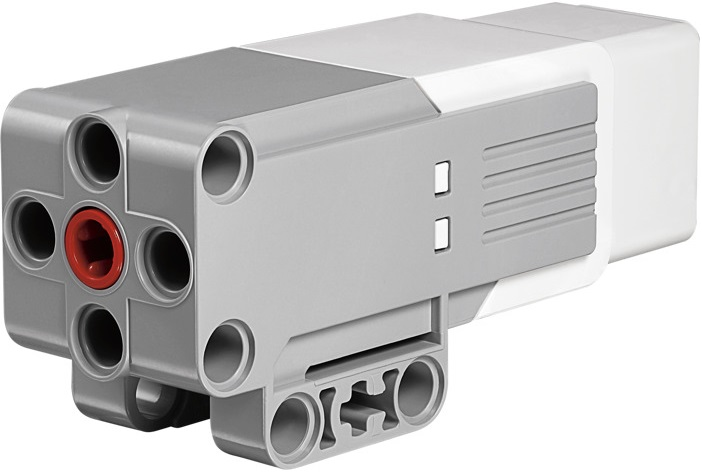
\includegraphics[width=3cm]{images/techAnalysis/LegoEV3MediumServomotor.jpg}
  \caption{LEGO MINDSTORMS EV3 medium servomotor \cite{BrickOWl-figure-EV3-mediumServo}}\label{fig:sssec:EV3MediumServomotor}
\end{figure}
In LEGO MINDSTORM, another type of servomotor, other than the large one, exists, namely the medium servomotor, which can be seen in \autoref{fig:sssec:EV3MediumServomotor}.
Like the large edition, this servomotor features a built-in rotation sensor, making it possible to control it within a single degree of accuracy.
The servomotor is also like the large servomotor powered through an RJ12 port, which it also uses to connect to the EV3.
The medium servomotor is with its maximum of 240-250rpm faster than the large servomotor, but is not as strong.
Like the large edition, the medium servomotor is compatible with both the LEGO MINDSTORMS EV3 brick and the LEGO MINDSTORMS NXT 2.0 brick \cite{lego_lego_EV3NXTCompatibility}.
\cite{LEGO_mindstorms_2013-1}
